\chapter{相关工作}
本文研究弱监督语义分割中的不确切监督和不准确监督,在不确切监督中,我们的研究重点是如何结合形状先验,在不准确监督中,我们关注如何利用分割标签的结构先验。本章介绍涉及到的四类相关工作:语义分割的不确切监督、自学习方法、降噪自编码器和语义分割中的不准确监督。

\section{语义分割的不确切监督}
为了降低标注成本,作为弱监督的一种类型,不确切监督采用粗粒度的标签,比如图像级别的标签(\cite{}),边界框(\cite{})和涂鸦式标签(\cite{})。该任务对提高数据标注的利用效率有重要意义。现有的方法大致可以分为两类,第一类采用迭代学习的框架,即先传播监督信息,生成伪标签,再用其训练模型。第二类方法应用基于正则项的训练框架,避免了生成伪标签的过程。接下来我们对这些工作进行详细介绍。


\citet{papandreou2015weakly}探索了在边界框和图像级标签这样弱标注训练数据的学习算法。该工作为弱监督的语义图像分割模型训练开发了期望最大化方法,来解决模型训练不足的问题。首先在标签标注成本上,收集图像中每个类别周围的边界框标注会比逐像素标注快大约15倍\citep{lin2014microsoft},收集图像级标签的标注成本更少。其次该文作者提出的期望最大化方法,在估计隐像素标签(被弱标签约束)和用随机梯度下降方法优化深度神经网络参数这两个阶段交替进行。

在图像级标签上,作者定义了该问题的概率图模型,并根据该模型,用期望最大化算法来从训练数据中学习模型参数,如图~\ref{c2_fig1}。考虑求期望阶段偏差的不同形式,作者提出了两种具体方法:EM-Fixed 和 EM-Adapt。在 EM-Fixed 中,根据图像级标签为每个像素设置固定的概率偏差,施加图像的前景区域约束。在 EM-Adapt 中,根据图像级标签设定前景区域面积的偏差,来对前景区域施加约束。

在边界框标签上,作者也探索了三种方法来训练分割模型:Bbox-Rect, Bbox-Seg 和 Bbox-EM-Fixed,如图~\ref{c2_fig2}。Bbox-Rect 采用了简单的标签赋值方法,在边界框内的像素全部设为目标类别的标签,在其外的则为背景标签。这种简单的方法会引入一些边界框内的假正类标签,为了解决这一问题,Bbox-Seg 被提出。具体做法是,在边界框内不再全部设为正类标签,而是选择一定比例的边界框中心区域设为正类标签,边界框外则全部设为负类标签,然后构建一个条件随机场来推理其他的标签。这两种利用边界框来估计分割图标签的方法,都可以看做是前处理步骤,随后利用生成标签来训练分割网络。此外,作者还提出了 Bbox-EM-Fixed,目标是在训练中改进分割标签估计,这是 EM-Fixed 的一个变种,不同的是仅对边界框内的像素施加前景偏差。最后这篇文章在 PASCAL VOC 2012 图像分割基准的评价指标有较高提升,验证了这些方法的有效性。


    \begin{figure*}[tbp]
        \centering 
        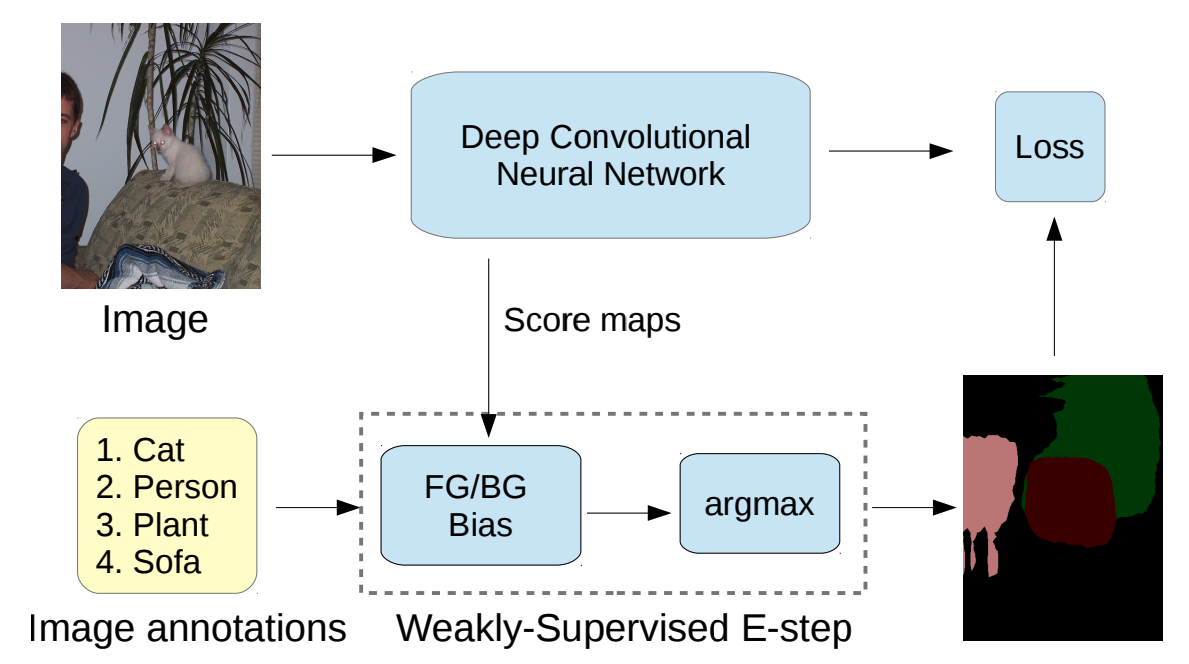
\includegraphics[width=1.0\textwidth]{img/c2/rel_a1.png}
        \bicaption{使用图像级标签的 DeepLab 模型训练过程。}{DeepLab model training using image-level labels.}
        \label{c2_fig1}
    \end{figure*}

    \begin{figure*}[tbp]
        \centering 
        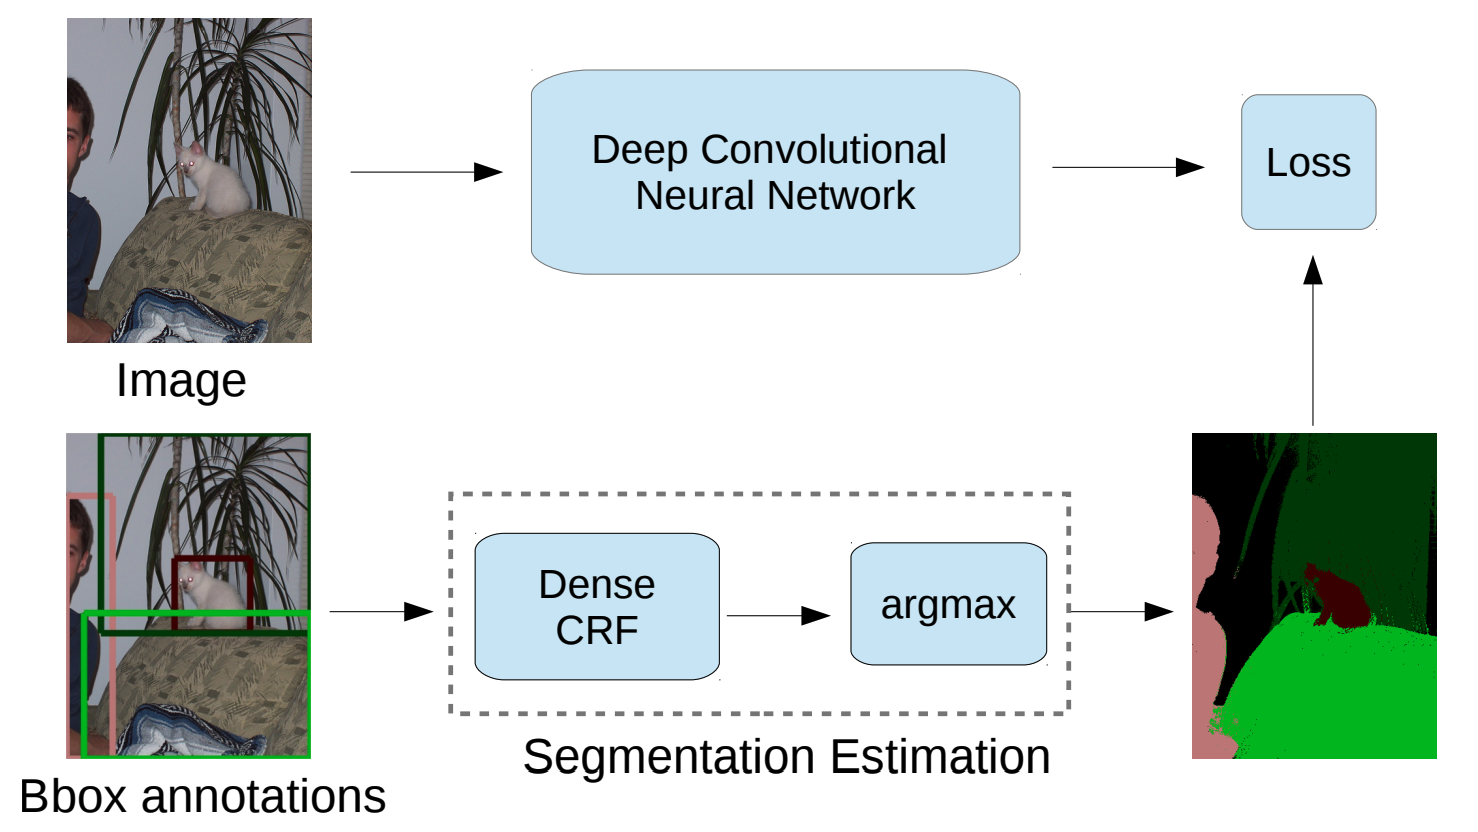
\includegraphics[width=1.0\textwidth]{img/c2/rel_a2.png}
        \bicaption{使用边界框标签的 DeepLab 模型训练过程。}{DeepLab model training from bounding boxes.}
        \label{c2_fig2}
    \end{figure*}

    \begin{figure*}[tbp]
        \centering 
        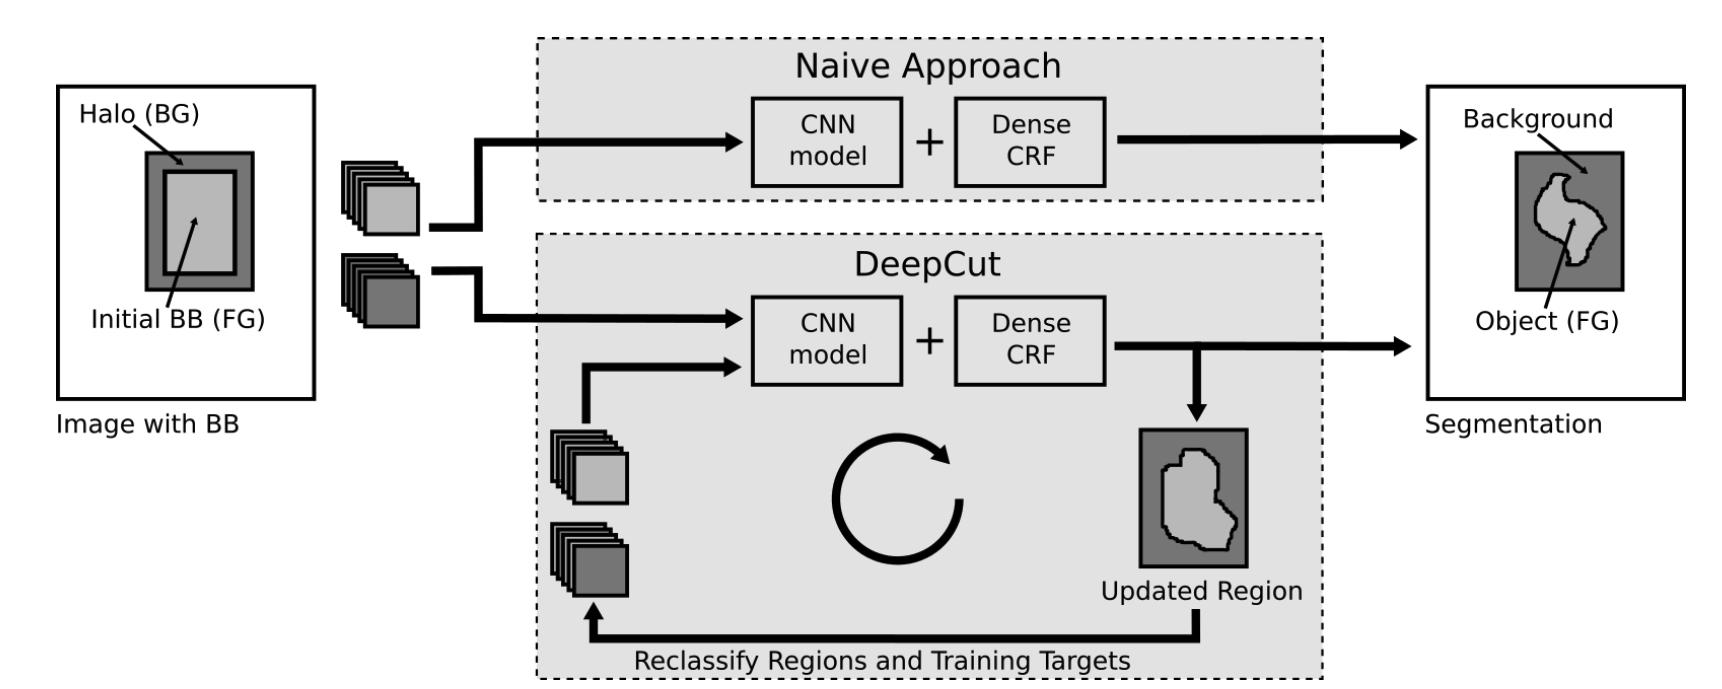
\includegraphics[width=1.0\textwidth]{img/c2/rel_a3.png}
        \bicaption{普通的 CNN 学习与提出的 DeepCut 方法的对比,后者迭代地更新学习目标。}{Naive CNN learning versus the proposed DeepCut approach, iteratively updating the learning target classes for input patches.}
        \label{c2_fig3}
    \end{figure*}

    \begin{figure*}[tbp]
        \centering 
        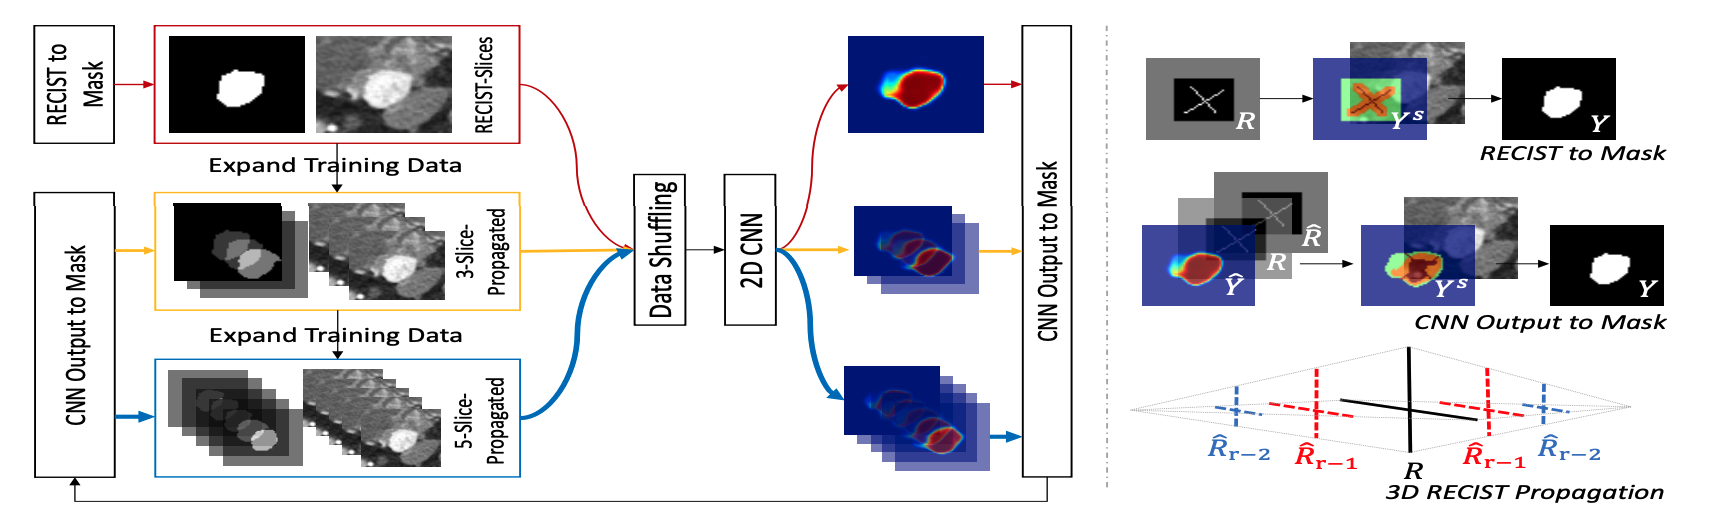
\includegraphics[width=1.0\textwidth]{img/c2/rel_a4.png}
        \bicaption{逐切片扩张的三维图像分割网络。}{The overview of slice-propagated 3D image segmentation network. }
        % 左侧图展示了训练图像的增加过程,每次邻近的图片连通生成的弱标签一起加入训练。右侧图展示了弱标签的传播过程,RECIST 标签通过 GrabCut 传播,未标注图像通过分割网络的预测传播得到标签。
        % Left: Each time adjacent slices are fed into the training process. Right: RECIST labels are initialized by GrabCut method, and CNN outputs are used to gradually generate extra training data for lesion segmentation.
        \label{c2_fig4}
    \end{figure*}


    \begin{figure*}[tbp]
        \centering 
        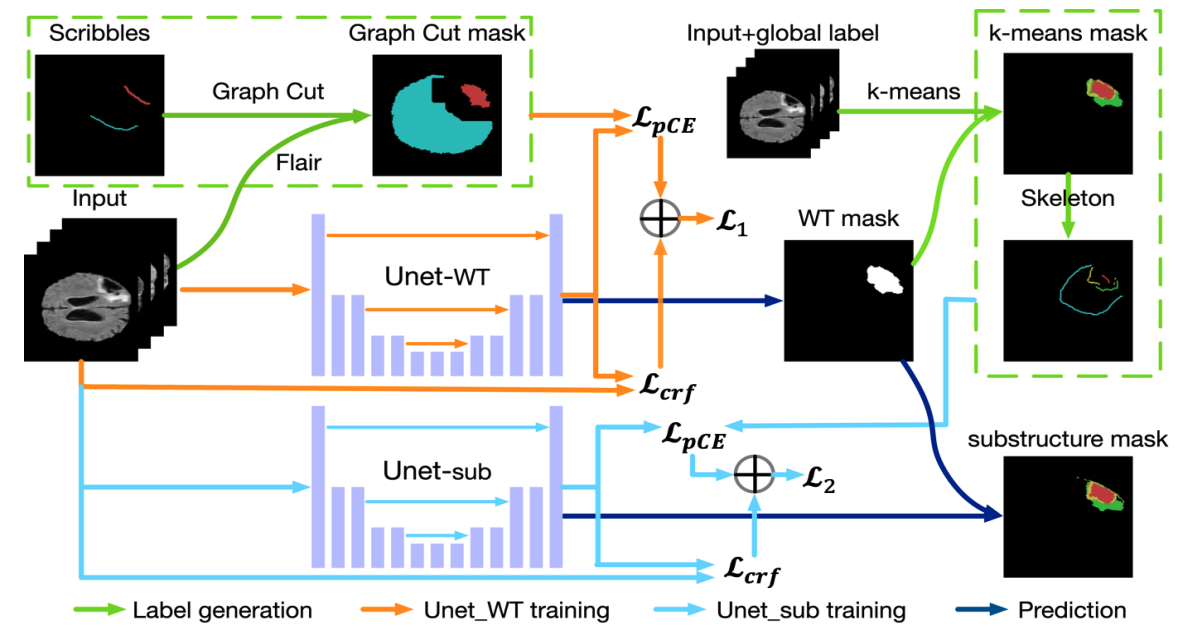
\includegraphics[width=1.0\textwidth]{img/c2/rel_a5.png}
        \bicaption{级联训练分割网络}{Workflow of the proposed cascaded method.}
        \label{c2_fig5}
    \end{figure*}


在 Deepcut\citep{rajchl2016deepcut}中进一步探讨了迭代地更新训练目标标签和模型参数的思想。该文的研究重点在边界框标签上。作者首先指出了边界框标签相对其他形式(比如涂鸦式)的优势,即对问题的空间约束(目标物体是完全包含在边界框内的),快速标注和轻量级存储(只需要定义对角线的两个端点)。本文目标是把神经网络模型和迭代的凸优化方法相结合,以从粗粒度的边界框标签恢复像素级物体分割。受 GrabCut 方法的启发,其用一个基于像素强度的图模型迭代地拟合图像区域,随后被正则化以得到分割。该文将此任务定义为稠密连接的条件随机场下的能量最小化问题,提出迭代地更新卷积网络学习的训练目标,并且应用全连接条件随机场来规范分割。

模型结构如图~\ref{c2_fig3},作者对比了普通的 CNN 训练方法和提出的 Deepcut 迭代方法。重要的区别在于,Deepcut 对训练目标的迭代更新,可以渐进地提高模型训练的效果,这种迭代提高的方法要优于单一不变的训练目标。具体实现上,论文中还提出了DeepCut方法的变体,并与其它算法在弱监督任务进行了比较。Deepcut 方法在 Fetal Magnetric Resonance Dataset\citep{damodaram2012foetal}的这两个分割任务上取得了不错的精度,超过了之前的方法。

在医学图像中,很多都是三维形态的,也可以看作一系列连续的二维医学图像的拼接。在三维图像上,标注成本更是大幅提高,基于弱标签的分割方法显得尤为重要。\citet{cai2018accurate}研究利用现有的 RECIST直径 标签来生成完整的三维图像分割结果。三维图像的 RECIST 标签只在中心一张二维切片上(RECIST 标签是在中心切片的物体内部画出一对相互垂直的长轴与短轴),这篇文章要解决两个主要挑战,一是有弱标注图像的标签传播,以训练有效的分割网络,二是从已标注图像到未标注图像的标签传播,来分割出完整的三维物体。对前一个问题,作者采用无监督方法来初始化标签,对后一个问题,则利用分割网络的预测结果,来自动生成可信的标签。作者用一个迭代扩张训练图像的过程,来覆盖整个待分割的三维图像。总的来说,这篇文章把三维图像分割分解成一系列二维图像分割任务,通过标签传播和分割模型的分阶段训练来生成分割结果,最后堆叠组合为三维分割结果。

分割过程如图~\ref{c2_fig4}所示,是一个基于卷积神经网络的逐切片传播的分割方法。首先,为有 RECIST 标注的切片初始化分割标签,然后用这些切片训练分割模型。其后,利用初步训练的模型给临近的未标注切片初始化分割标签,用扩张后的切片及标签继续训练模型。这个过程不断迭代,直至所有切片都加入训练。作者在淋巴结数据集和\citep{roth2014new} DeepLesion 数据集\citep{yan2018deep}进行实验,表明了所提出方法的优良性能。

另一方面,有些组织由多个子区域构成,比如脑肿瘤可能由两到三种子区域,每个子区域都需要单独分割。如果每个子区域进行标注,成本也会较大。\citet{ji2019scribble}为这种任务提出了一种结合两种弱标签形式的标注方法,来减少标注成本。这种混合标注策略是,对整体的肿瘤区域用涂鸦式标签,对各个子区域是否存在给出的全局图像级标签。这种方式下,整体的肿瘤区域通过涂鸦式标签来学习,图像级标签用来引导子区域的聚类。这篇文章提出通过级联模型的方式,来解决这样具有层次结构的分割任务。

模型如图~\ref{c2_fig5}。受之前的级联网络的启发,这个模型采用先训练整体肿瘤分割,再子区域分割的方式。具体地,作者先用涂鸦式标签和由其初始化得到的图割标签,来训练整体肿瘤的分割网络。之后再在图像级标签的引导下,用无监督聚类方法提取肿瘤的各个子区域。最后把聚类得到的标签作为弱标签,来训练第二个子区域分割网络。作者还在分割网络训练中加入了 Dense CRF Loss,来提高分割边缘的连续性与准确性。这种方法在 BraTS2017 数据集上进行了评估,在整体肿瘤分割和子区域分割上都取得了接近全监督上限的结果。

以上方法有共同之处:都是利用推理方法(GrabCut、CRF或初始化模型推理)来显式地生成全标签,然后使用某种处理机制来用生成的标签训练模型。除了显式地生成伪标签再训练,另一类方法是直接利用弱标签训练,通过施加先验正则项来约束训练,以求较好的训练结果。\citet{kervadec2020bounding}和\citet{tang2018regularized}是近期的重要工作。

\citet{kervadec2020bounding} 采用边界框标签,提出了一种基于全局约束的弱监督分割方法。作者首先提出了边界框的拓扑先验,包括框内的紧致性先验、框外的全背景先验和前景区域尺寸先验,这些先验被作为约束条件加入模型的训练目标。不过这些先验是不等式形式的约束,为了直接训练,作者通过对数障碍惩罚函数把不等式约束处理为损失函数的形式。这种利用全局约束来解决弱监督问题的方法,充分利用了领域先验知识,避免了只有少量标签训练的结果不确定性。并且基于约束方法能实现端到端的训练,可以避免显式生成伪标签过程中的错误传播。
    \begin{figure*}[tbp]
        \centering 
        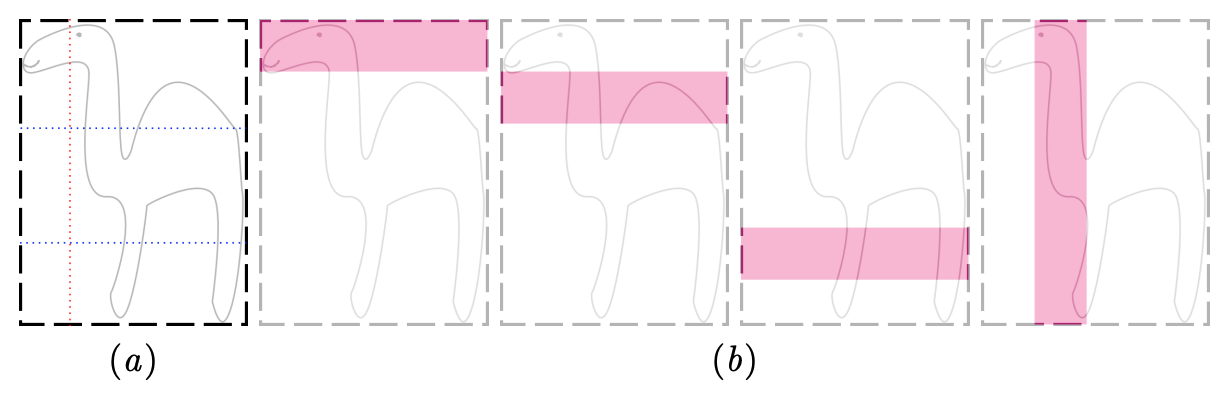
\includegraphics[width=1.0\textwidth]{img/c2/rel_a6.png}
        \bicaption{边界框标签的紧致性先验示意图:(a) 任一条竖直或水平的线段至少与一个前景像素相交。 (b) 更广泛地,宽度为 w 的线段至少与 w 个前景像素相交}{Illustration of the tightness prior: (a) any vertical (red) or horizontal (blue) line will cross at least one pixel of the camel. (b) This can be generalized, where segments of width w cross at least w pixels of camel.}
        \label{c2_fig6}
    \end{figure*}
全局约束充分考虑利用弱标签的信息。紧致性先验如图~\ref{c2_fig6}所示,基于边界框紧致地包围着目标物体边界,在框内的任意一条水平或竖直线段都会至少与一个像素相交。这种先验约束,能够防止训练过程中过拟合到背景类别而前景预测失败的问题。全背景先验是指边界框外的区域都是背景类别,约束了前景的空间区域。前景区域尺寸先验,则是指目标物体在框内的面积比例有先验的下界与上界,利用尺寸先验可以约束分割结果的区域比例关系。这些全局先验通过对数障碍惩罚函数转换为标准的损失函数形式,可以直接使用随机梯度下降方法进行优化。
这篇文章在两个不同的公开数据集 PROMISE12\citep{Litjens2014EvaluationOP}和 ATLAS\citep{Liew2018ALO}进行试验,结果表明,这种方法可以接近全监督的分割效果,并且显著超过之前的 DeepCut 方法,同时避免了显式生成伪标签的耗时计算。

\citet{tang2018regularized}则在涂鸦式标签上探索把正则项融入损失函数,以实现浅层分割的效果(如图割法或 Dense CRF)。这篇文章通过设计 MRF/CRF 形式的约束项,来为分割模型引入浅层分割的特性如连续性、相关性、空间关系等。这种隐式的约束方法简化了弱监督的训练,避免了额外的 MRF/CRF 推理步骤来生辰伪标签,提高了训练的质量和效率。这篇文章提出了集中用于弱监督的正则损失,分别是基于 Potts、Dense CRF 和 Kernelcut 的正则。作者通过 PASCAL VOC12 的实验对比了早期的显式推理步骤和不同正则损失函数,验证了所提出方法在弱监督语义分割的接近全监督的效果。


\section{自学习方法}
训练数据的缺乏是学习中的常见问题,自学习方法有望作为一种解决方案。
自学习方法通过___

\citet{Raina}


\citet{Li}


\citet{Bazzani}



\section{降噪自编码器}
降噪自编码器将图像编码到高维空间的一个隐向量,该向量对噪声具有不变性,可以表示原始图像。

\citet{Vincent}


\citet{Sundermeyer}



\section{语义分割的不准确监督}
不准确监督作为弱监督的另一种类型,面临着标签中有一部分错误的问题,即噪声标签问题。如何有效利用好噪声标签,来训练得到鲁棒的语义分割网络,是该任务的核心问题。近来已有一些工作在该任务上做了探索,并取得了一些进展。

\citet{Zhu}


\citet{Xue}


\citet{CL}


\citet{Tri-network}
 


\section{本章小结}
本章中我们对相关的工作进行了总结并分析,包括语义分割中的不确切监督、自学习方法、降噪自编码器、不准确监督等部分。为开展我们的研究工作奠定基础。

